%This should introduce the motivation behind the research undertaken for the project, providing background material that is relevant to the problem(s) being addressed. It is important you also indicate the area/discipline where the research sits and how it aligns with the degree programme you are enrolled on.

% goal ~1k words
% actual 1642 words

In many stories of science-fiction, there are robots that are intelligent, borderline human in the way they talk, the way they walk, and the way they interact with their environments. Famous examples of this are C-3PO from Star Wars, Sunny from I-Robot, and Wall-E for the eponymous Disney animation. These kinds of robots seem to be creatures that won't exist any time soon, and they probably won't, but with every advancement in the field of robotics and autonomous systems, we step closer to that reality.\\
One of the most key human senses, which provides a way for a robot to effectively communicate with and understand the real world, is sight. As with human vision, which is essential in interpreting and acting upon the surrounding world, so seeing confers a whole range of possibilities upon a machine. Computer vision is an area of robotics, dedicated to providing machines with the sense of sight. The computing of visual information, identification of objects, and consequent decision-making in respect to the environment bring us closer to the intelligent, interactive robots that have long been envisioned in science fiction.

\section{Background}
    Human Pose Estimation (HPE) research started when computer vision gained popularity in the late 1960s and early 1970s. Scientists first focused on basic problems like as shape analysis, object recognition, and visual understanding. As computer vision developed, HPE became a stand-alone area of study \citep{Roboflow}. Historically, HPE was frequently described probabilistically to account for likely inference ambiguities. Since deep learning has been more widely used, the focus has switched to end-to-end trainable models because of their ability to extract intricate patterns and postures from data. Traditionally, computer vision systems have assessed an object's or person's posture by geometric calculations and feature-based techniques. But, the biggest developments in HPE came with the advent of deep neural networks, convolutional neural networks, and computer vision. The field has advanced considerably in spite of these challenges, and more recent techniques that make use of properly designed neural networks may provide amazing results in challenging scenarios involving a large number of, perhaps veiled, interacting individuals \citep{liu2018recognizing}. Now that these detections have the necessary technology and are sufficiently precise, they may be employed for commercial purposes. It also offers a wealth of new application potential and signifies a major change in HPE's overall direction.\\
    The HPE innovations unlock the potential for using state-of-the-art computer vision technologies within physical training and, hence, change the way athletes and fitness enthusiasts everywhere can improve their performance.\\
    The use of technology in physical training has transformed the way athletes and fitness enthusiasts approach their routines in recent years. Although traditional coaching techniques have long been successful in directing athletes, they can be improved by utilising the accuracy and instantaneous feedback that contemporary technology offers. The creation of computer-vision based training coaches, which use cutting-edge algorithms and machine learning to assess and improve physical performance, has been made possible by this gap. \citep{debnath2022review}\\
    The automatic extraction, analysis, and comprehension of meaningful information from a single image or a set of images is the focus of the computer vision area of artificial intelligence. Computer vision systems can precisely track and evaluate motions made during physical exercise, providing instantaneous feedback and coaching in real time. This technology helps prevent accidents in addition to assisting with form and technique modification by identifying improper actions. \citep{borisov2023application}\\
    Thanks to developments in wearable technology and high-definition cameras, computer vision based training systems are now easy to utilise. These gadgets can record precise movement data, which is evaluated by astute algorithms to produce valuable results. Thus, training regimens that are especially designed for athletes and adjust to their unique demands and development may be beneficial.\\
    Furthermore, the COVID-19 epidemic has sped up the transition in a number of industries, including sports and fitness, towards remote and digital solutions. The need for online coaching and training resources has increased as a result of lockdowns and social distancing. As a workable alternative, computer-vision based training instructors let customers to continue their exercise regimens under the supervision of professionals from the comfort of their own homes. It is important to note that this is not intended as a replacement for professional coaches, rather as an aid for them to have better effectivness.

\section{Area of Research}
    HPE is an area of research within computer vision that aims to teach robots how to make sense of the human form and the motions it is capable of performing. It involves the identification and classification of the joints in the human body, capturing a set of coordinates for each joint, known as a key point, that can describe the pose of a person. HPE has a wide set of uses in many fields: In games, with motion capture technologies reliant on HPE, it allows developers to encode more realistic and fluid character movements. In healthcare, healthcare providers can monitor a patient's movements and detect any abnormalities. Augmented reality, allows the user to interact with the digital content in more natural and intuitive ways with gestures. And finally, the use-case that is the primary focus of this project, is sports training. HPE can be used to analyse a user's performance, identify areas for improvement, and develop personalised training programs based on the physical level of the user. For example, HPE could be used to analyse a runner's form, e.g. How straight is their back? What part of the foot are they landing on? Are they leaning more to one side or landing more heavily on one foot?..., and provide feedback on how to improve their technique. HPE can be used to collect data about any exercises where the movement of the body is vital to its effectiveness.
    
\section{Motivation}
    Over the last few decades, the percentage of people who are either overweight or obese has steadily increased. This is a concerning trend as being obese increases the risk of many other health conditions such as type 2 diabetes, coronary heart disease, some types of cancer, and stroke \parencite{NHS-obesity}. As seen in Figure~\ref{fig:obesity}, over 60\% of the UK population is considered overweight or obese. \\

    \begin{figure}[htbp]
        \centering
        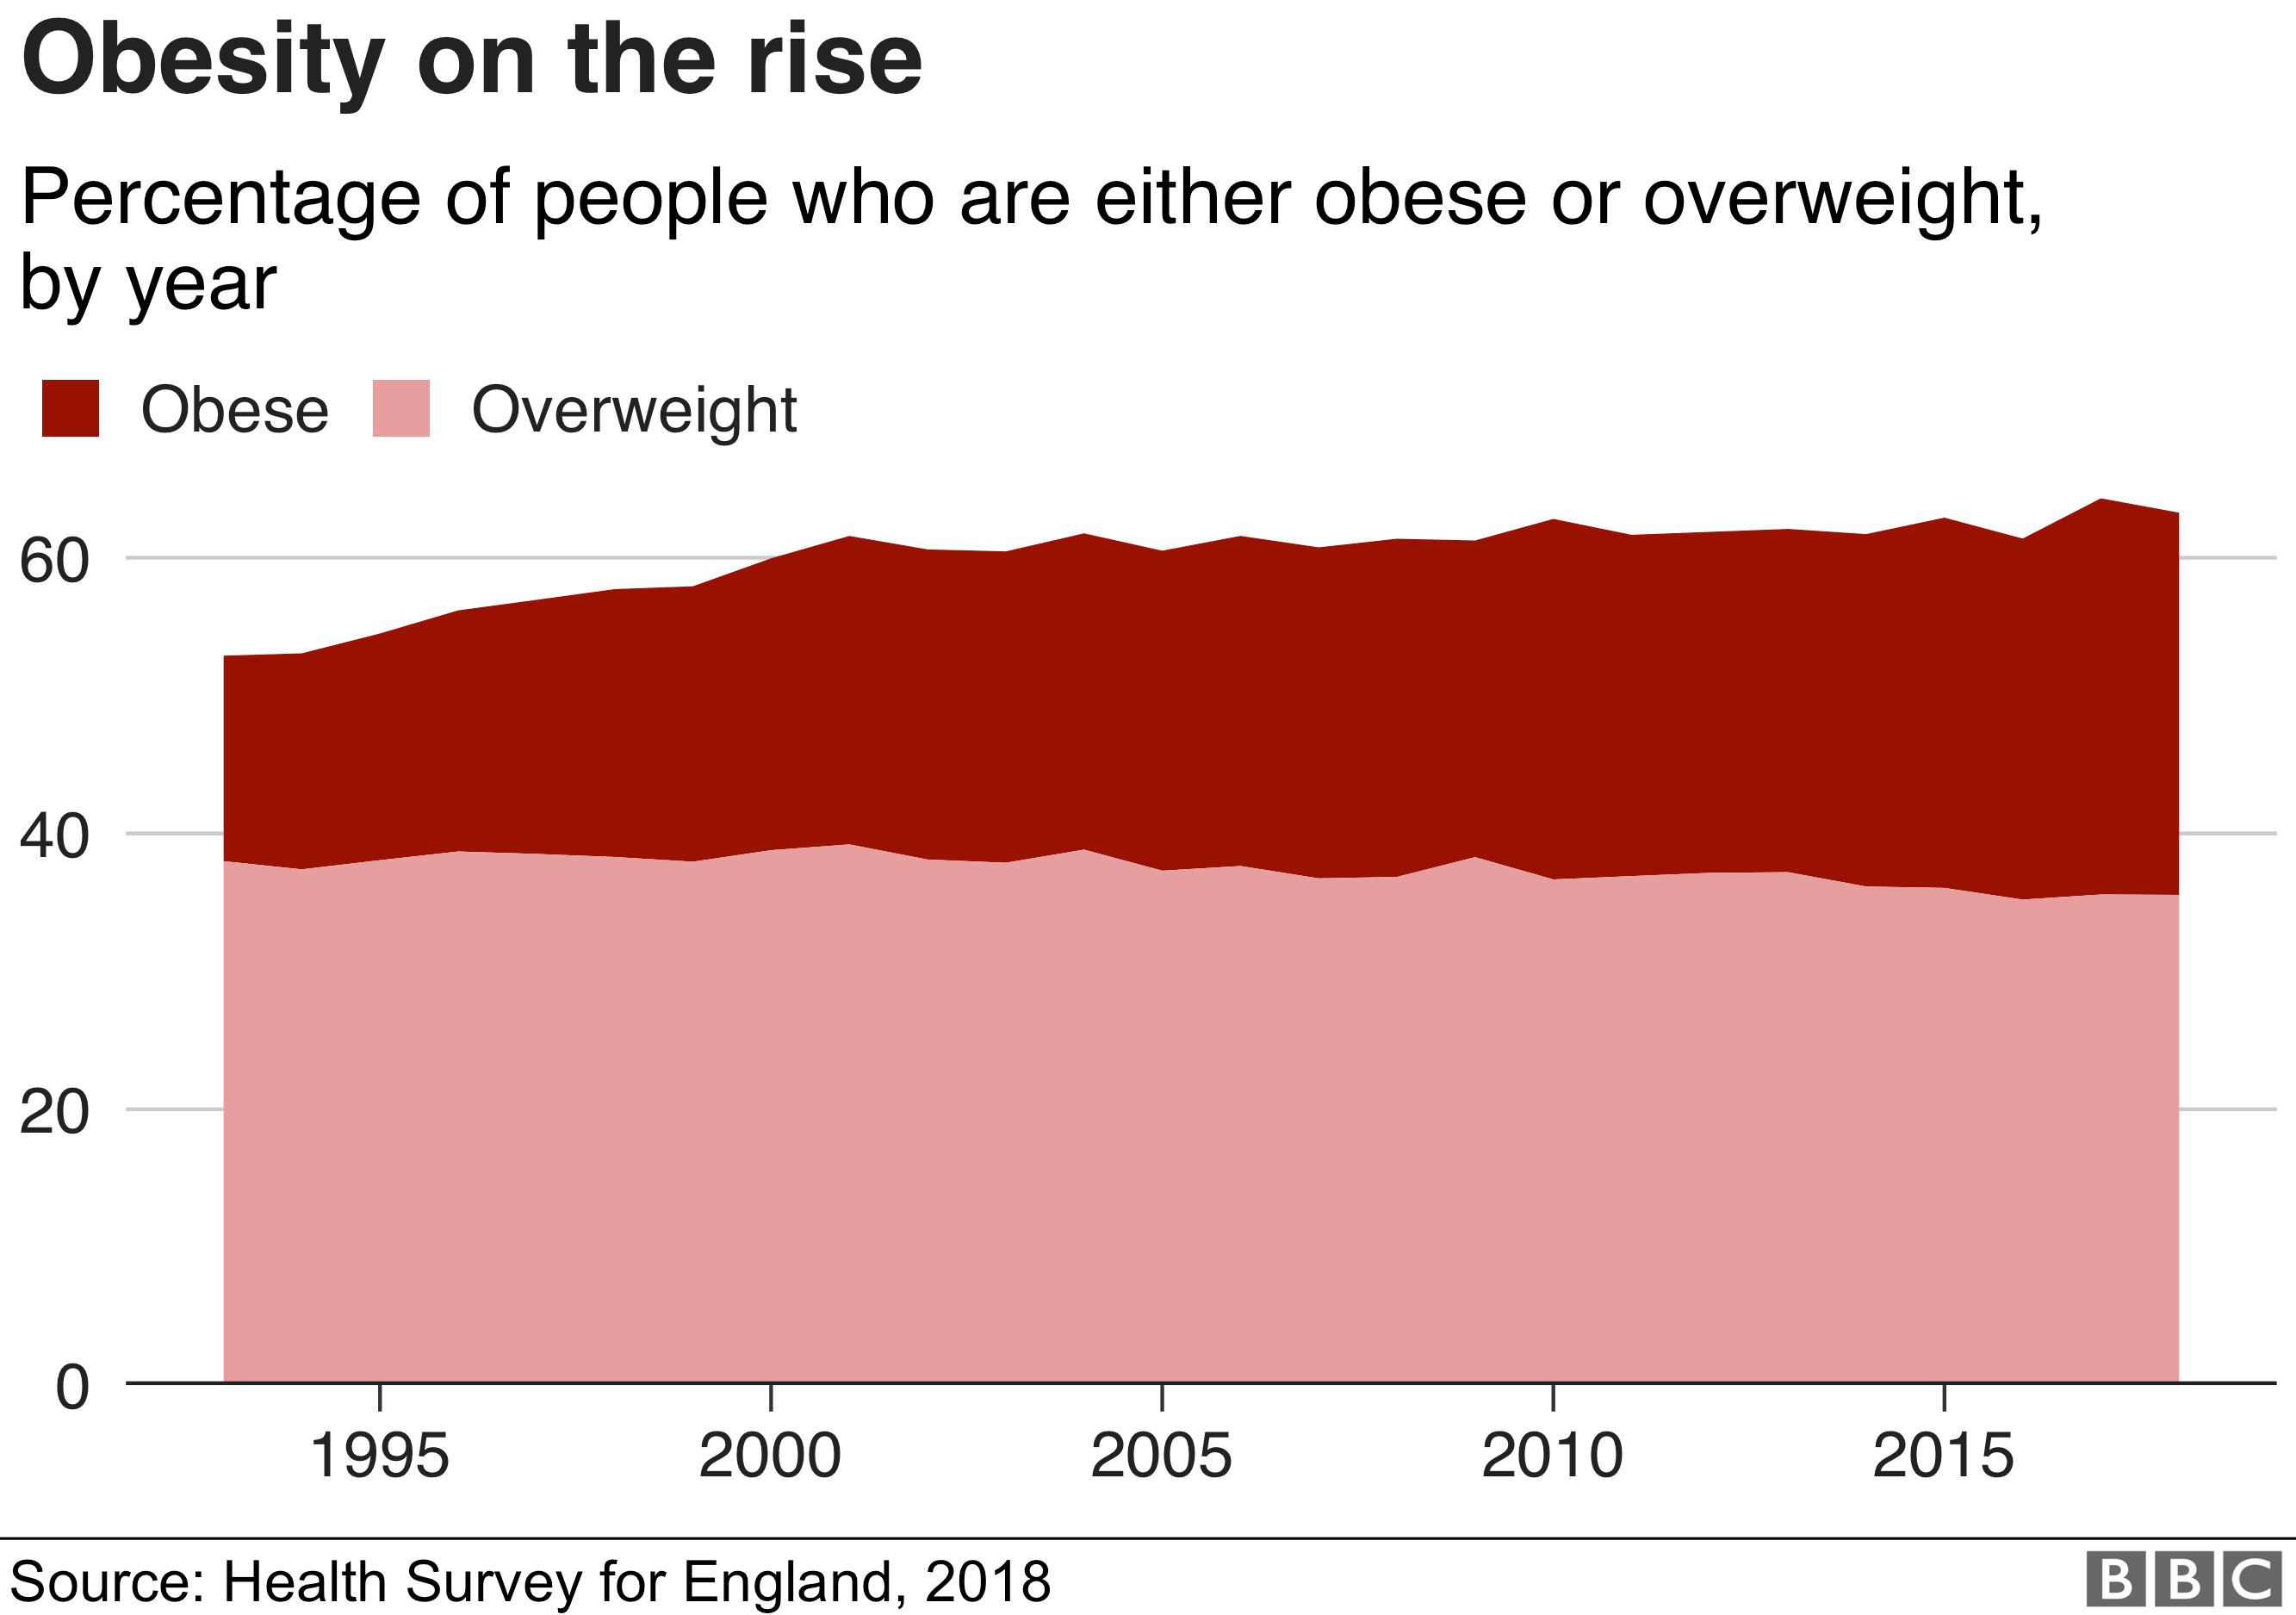
\includegraphics[width=0.67\textwidth]{figures/obesity.png}
        \caption{Percentage of people who are either obese or overweight, by year (Source: Health Survey for England, 2018)}\label{fig:obesity}
    \end{figure}

    To help solve that issue, it is important to encourage people to workout, but going to the gym can be daunting, especially when you don't know how to perform exercises properly. Creating an AI personal trainer will give people the knowledge and confidence to exercise more at home or the gym. Furthermore, exercise has many benefits other than weight loss, it reduces the risk of the issues mentioned above and has been shown to improve mental health \parencite{NHS-benefits}.\\
    

\section{Problem Statement}
    It is difficult to obtain real-time, individualised input for physical exercise, especially when it is done remotely. Exercise enhances both mental and physical health, but without the right supervision, people run the danger of getting hurt and don't obtain the full benefits of working out. The necessity for remote training solutions has been made evident by the COVID-19 outbreak increasing the popularity of working out at home instead of at the gym. Accurate, real-time feedback can be given by a computer-vision based training coach, which can enhance training, reduce the risk of injury, and promote mental health.

    
\section{Scope of the Project} 
    This project aims to create a program that will act as a personal trainer and that will track the mood of the user to determine the effect of physical exercise on acute mood. This means using a computer vision human pose estimator to find the landmarks on the user's body to determine their shape while asking them about their mood before and after an exercise session. This project will not use any deep learning methods to train any models for the recommendation system and repetition counter as no exercise data will be collect due to time constraints. Simple mathematical methods will be applied instead. The only data that will be collected will be user feedback solely for the purpose of evaluating the performance of the program.
    
\section{Structure of the Thesis}
    The structure of the thesis will proceed as follows. First I will perform a literature review of related work about the different uses of Computer Vision methods, this will include reviewing object detection, object segmentation, human pose estimation, and motion capture. I will also quickly review papers that explore the link between physical exercise and its effect on mood and mental health.\\
    Based on the findings from the literature review, I will lay out my aims and objectives for this project with the goal of having them be novel and have little previous research. These aims and objectives will be Specific, Measurable, Assignable, Realistic and Time-related as per the SMART principles.\\
    Following that, I will describe the methodology of the project, outlining the research design, the architecture of the system, the selection of the algorithm, the development environment including the tools and software used and the version control, the ethical considerations of the project, and an analysis of the risks that will potentially be faced.\\
    Subsequently, I will detail how I implemented the program, first by specifying the system requirements (both software and hardware), then I'll move on to recounting of the creation of the application by describing the integration of the model and the real-time processing.\\
    After the creation of the application, this is the creation of the Graphical User Interface (GUI) going through the development of both the frontend and the backend.\\
    The final section necessary for the detailing of the implementation is the testing and debugging with unit testing and integration testing.\\
    For the penultimate chapter, I will evaluate the performance in results and discussion. In this chapter, I will compare this project with existing solution, I will ponder the user feedback from the usability testing, I will go over the limitations of this project, and finally, provide my interpretation of the results.\\
    And Finally, to conclude, I will summarise the findings, describe the contributions to the field, explain the practical implications, make recommendations for future work, and provide my final thoughts on the entire project.